\documentclass[12pt,a4paper,oneside]{report}

\usepackage[a4paper,top=2.5cm,bottom=2.5cm,left=3cm,right=2cm]{geometry}
\usepackage{fontspec}
\usepackage{graphicx}
\usepackage{float}
\usepackage{array}
\usepackage{booktabs}
\usepackage{longtable}
\usepackage{amsmath}
\usepackage{amssymb}
\usepackage{enumitem}
\usepackage{titlesec}
\usepackage{xcolor}
\usepackage[hidelinks]{hyperref}

\IfFontExistsTF{Times New Roman}
    {\setmainfont{Times New Roman}}
    {\setmainfont{TeX Gyre Termes}}
\IfFontExistsTF{Consolas}
    {\setmonofont{Consolas}}
    {\setmonofont{Latin Modern Mono}}
\graphicspath{{../}{../Dataset/}}
\setlength{\parindent}{1.25cm}
\setlength{\parskip}{0.25em}
\renewcommand{\baselinestretch}{1.2}

\titleformat{\chapter}[hang]{\bfseries\Large}{Chương \thechapter.}{0.6em}{}
\titleformat{\section}{\bfseries\large}{\thesection}{0.6em}{}
\titleformat{\subsection}{\bfseries\normalsize}{\thesubsection}{0.6em}{}

\newcommand{\studentname}{Nguyễn Trọng Hiệp}
\newcommand{\studentid}{\textit{Điền MSSV}}
\newcommand{\classname}{\textit{Điền lớp}}
\newcommand{\supervisor}{\textit{Điền tên giảng viên hướng dẫn}}
\newcommand{\thesistitle}{Xây dựng ứng dụng phát hiện gù lưng và nhắc nhở tư thế ngồi bằng thị giác máy tính}

\begin{document}

\begin{titlepage}
    \centering
    {\bfseries ĐẠI HỌC BÁCH KHOA HÀ NỘI\par}
    {\bfseries TRƯỜNG CÔNG NGHỆ THÔNG TIN VÀ TRUYỀN THÔNG\par}
    \vspace{2.5cm}

    {\bfseries\Large BÁO CÁO ĐỒ ÁN TỐT NGHIỆP\par}
    \vspace{1.2cm}
    {\bfseries\Large \thesistitle\par}
    \vspace{2.2cm}

    \begin{tabular}{>{\bfseries}p{5cm}p{8cm}}
        Sinh viên thực hiện: & \studentname \\
        Mã số sinh viên: & \studentid \\
        Lớp: & \classname \\
        Giảng viên hướng dẫn: & \supervisor \\
    \end{tabular}

    \vfill
    {\bfseries Hà Nội, 2026\par}
\end{titlepage}

\chapter*{Lời cam đoan}
Tôi cam đoan báo cáo này được thực hiện dựa trên quá trình tìm hiểu, thiết kế và cài đặt ứng dụng phát hiện tư thế gù lưng của bản thân. Các tài liệu, công nghệ và thư viện được sử dụng trong đồ án đều được nêu rõ trong phần tài liệu tham khảo.

\chapter*{Lời cảm ơn}
Em xin cảm ơn giảng viên hướng dẫn đã hỗ trợ, góp ý trong quá trình thực hiện đồ án. Em cũng xin cảm ơn gia đình và bạn bè đã động viên, tạo điều kiện để em hoàn thành sản phẩm và báo cáo này.

\chapter*{Tóm tắt}
Đồ án xây dựng một ứng dụng theo dõi tư thế ngồi theo thời gian thực, sử dụng webcam, MediaPipe Pose Landmarker và giao diện PySide6. Hệ thống hiệu chuẩn tư thế chuẩn của người dùng, sau đó so sánh các đặc trưng hình học như độ cao vai, khoảng cách mũi--vai, độ rộng vai và độ rộng khuôn mặt để nhận biết các trạng thái: tư thế tốt, hơi cúi, gù/cúi rõ, hơi ngả sau và ngả sau. Khi phát hiện tư thế xấu liên tục, ứng dụng hiển thị nhắc nhở và có thể phát âm thanh hoặc làm mờ màn hình.

\textbf{Từ khóa:} phát hiện tư thế, gù lưng, MediaPipe, OpenCV, PySide6, thị giác máy tính.

\tableofcontents

\chapter{Giới thiệu}

\section{Bối cảnh}
Thói quen ngồi lâu trước máy tính làm tăng nguy cơ đau cổ, đau lưng và sai lệch tư thế. Các giải pháp nhắc nhở truyền thống thường dựa trên thời gian cố định, chưa phản ánh trực tiếp trạng thái cơ thể của người dùng. Vì vậy, một hệ thống theo dõi tư thế bằng webcam có thể đưa ra cảnh báo phù hợp hơn, đặc biệt trong môi trường học tập và làm việc cá nhân.

\section{Mục tiêu}
Đồ án hướng tới các mục tiêu chính sau:
\begin{itemize}[leftmargin=1.2cm]
    \item Phát hiện khung xương cơ thể từ ảnh webcam theo thời gian thực.
    \item Hiệu chuẩn tư thế chuẩn riêng cho từng người dùng.
    \item Phân loại tư thế dựa trên các đặc trưng hình học đơn giản, dễ giải thích.
    \item Xây dựng giao diện desktop cho phép theo dõi, hiệu chuẩn lại và cấu hình nhắc nhở.
\end{itemize}

\section{Phạm vi}
Hệ thống tập trung vào tư thế thân trên khi người dùng ngồi trước webcam. Đồ án không nhằm thay thế thiết bị y tế hoặc chẩn đoán bệnh lý cột sống; kết quả chỉ có ý nghĩa hỗ trợ nhắc nhở tư thế trong sử dụng hằng ngày.

\chapter{Cơ sở lý thuyết và công nghệ sử dụng}

\section{Phát hiện điểm mốc cơ thể}
MediaPipe Pose Landmarker cung cấp tập các điểm mốc cơ thể đã chuẩn hóa theo khung hình. Trong đồ án, các điểm quan trọng gồm mũi, hai vai và hai tai. Từ các điểm này, hệ thống suy ra sự thay đổi của phần thân trên khi người dùng cúi về trước hoặc ngả về sau.

\section{Đặc trưng hình học}
Các đặc trưng được trích xuất từ điểm mốc gồm:
\begin{itemize}[leftmargin=1.2cm]
    \item $shoulder\_y$: tung độ trung bình của hai vai.
    \item $nose\_dist$: khoảng cách theo trục dọc giữa mũi và đường vai.
    \item $shoulder\_width$: khoảng cách ngang giữa hai vai.
    \item $face\_width$: khoảng cách ngang giữa hai tai.
\end{itemize}

Trong giai đoạn hiệu chuẩn, người dùng ngồi thẳng trong vài giây. Hệ thống lấy trung bình các đặc trưng này để tạo giá trị nền. Ở mỗi khung hình sau đó, các tỷ lệ được tính như sau:
\begin{align}
    shoulder\_drop &= current\_shoulder\_y - baseline\_shoulder\_y, \\
    nose\_ratio &= \frac{current\_nose\_dist}{baseline\_nose\_dist}, \\
    shoulder\_width\_ratio &= \frac{current\_shoulder\_width}{baseline\_shoulder\_width}, \\
    face\_width\_ratio &= \frac{current\_face\_width}{baseline\_face\_width}.
\end{align}

\section{Công nghệ sử dụng}
\begin{longtable}{p{4cm}p{10cm}}
    \toprule
    \textbf{Công nghệ} & \textbf{Vai trò trong hệ thống} \\
    \midrule
    Python & Ngôn ngữ cài đặt chính. \\
    OpenCV & Đọc ảnh từ webcam, xử lý khung hình và vẽ kết quả. \\
    MediaPipe & Phát hiện điểm mốc cơ thể theo thời gian thực. \\
    PySide6 & Xây dựng giao diện desktop, hộp thoại cảnh báo và cấu hình. \\
    Qt Multimedia & Phát âm thanh nhắc nhở khi phát hiện tư thế xấu liên tục. \\
    \bottomrule
\end{longtable}

\chapter{Phân tích và thiết kế hệ thống}

\section{Yêu cầu chức năng}
Ứng dụng cần hỗ trợ các chức năng sau:
\begin{itemize}[leftmargin=1.2cm]
    \item Tự động mở camera và hiển thị khung hình theo thời gian thực.
    \item Hiệu chuẩn tư thế chuẩn trong khoảng 3 giây.
    \item Phân loại tư thế hiện tại và hiển thị trạng thái trực quan.
    \item Cho phép hiệu chuẩn lại khi người dùng thay đổi vị trí ngồi.
    \item Cảnh báo khi tư thế xấu kéo dài quá thời gian cấu hình.
    \item Cho phép chạy nền bằng system tray.
\end{itemize}

\section{Kiến trúc tổng thể}
Hệ thống được chia thành ba nhóm thành phần chính:
\begin{itemize}[leftmargin=1.2cm]
    \item \textbf{Tầng thu nhận dữ liệu}: đọc webcam bằng OpenCV, chuyển đổi khung hình sang định dạng phù hợp cho MediaPipe.
    \item \textbf{Tầng xử lý}: phát hiện pose, trích xuất đặc trưng, hiệu chuẩn và phân loại tư thế.
    \item \textbf{Tầng giao diện}: hiển thị video, trạng thái, nút điều khiển, cấu hình cảnh báo và nhắc nhở.
\end{itemize}

\section{Luồng xử lý}
Quy trình hoạt động của ứng dụng gồm các bước:
\begin{enumerate}[leftmargin=1.2cm]
    \item Khởi tạo mô hình MediaPipe Pose Landmarker và camera.
    \item Người dùng ngồi thẳng để hệ thống thu thập giá trị nền.
    \item Với mỗi khung hình, hệ thống phát hiện điểm mốc cơ thể.
    \item Trích xuất các đặc trưng hình học từ mũi, vai và tai.
    \item So sánh với giá trị nền để phân loại tư thế.
    \item Nếu tư thế xấu kéo dài, kích hoạt cảnh báo.
\end{enumerate}

\chapter{Cài đặt}

\section{Mô-đun thuật toán}
Mô-đun thuật toán được cài đặt trong các hàm xử lý điểm mốc và hàm \texttt{classify\_posture}. Các điểm mốc được sử dụng trực tiếp từ MediaPipe, sau đó chuyển thành đặc trưng hình học. Cách tiếp cận này có ưu điểm là nhẹ, dễ chạy thời gian thực và không cần huấn luyện mô hình riêng.

Các ngưỡng chính trong phiên bản hiện tại:
\begin{longtable}{p{6cm}p{7cm}}
    \toprule
    \textbf{Điều kiện} & \textbf{Ý nghĩa} \\
    \midrule
    $shoulder\_width\_ratio < 0.82$ và $face\_width\_ratio < 0.82$ & Ngả sau rõ. \\
    $shoulder\_width\_ratio < 0.90$ hoặc $face\_width\_ratio < 0.90$ & Hơi ngả sau. \\
    $shoulder\_drop > 0.06$ & Vai tụt xuống rõ so với tư thế chuẩn. \\
    $shoulder\_drop > 0.035$ & Vai tụt nhẹ. \\
    $nose\_ratio < 0.75$ & Mũi gần vai rõ, dấu hiệu cúi/gù. \\
    $nose\_ratio < 0.866$ & Cúi nhẹ. \\
    \bottomrule
\end{longtable}

\section{Mô-đun giao diện}
Giao diện chính được xây dựng bằng PySide6. Luồng xử lý camera chạy trong \texttt{QThread} để không làm treo giao diện. Các tín hiệu Qt được dùng để gửi khung hình và trạng thái từ luồng xử lý sang cửa sổ chính.

Cửa sổ ứng dụng gồm vùng xem camera và bảng điều khiển. Người dùng có thể bắt đầu/dừng theo dõi, hiệu chuẩn lại, thay đổi độ nhạy, cấu hình hành động cảnh báo và ẩn ứng dụng xuống system tray.

\begin{figure}[H]
    \centering
    \IfFileExists{../image.png}{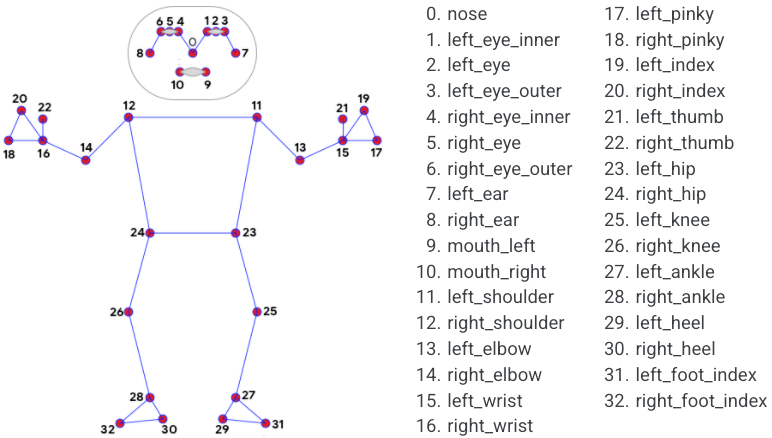
\includegraphics[width=0.78\textwidth]{../image.png}}{\fbox{\parbox{0.78\textwidth}{Chưa có ảnh minh họa giao diện.}}}
    \caption{Minh họa giao diện hoặc kết quả xử lý của ứng dụng}
    \label{fig:app-ui}
\end{figure}

\section{Cơ chế cảnh báo}
Hệ thống không cảnh báo ngay khi phát hiện một khung hình xấu, mà theo dõi trạng thái xấu liên tục trong một khoảng thời gian. Cách làm này giúp giảm cảnh báo nhầm khi người dùng chỉ cử động ngắn. Khi vượt ngưỡng thời gian, ứng dụng có thể hiển thị hộp thoại, phát âm thanh, làm mờ màn hình và gửi thông báo qua system tray.

\chapter{Thử nghiệm và đánh giá}

\section{Bộ dữ liệu thử nghiệm}
Bộ dữ liệu thử nghiệm trong thư mục \texttt{Dataset} gồm 24 ảnh tĩnh, được đặt tên theo người chụp và nhãn tư thế. Các nhãn được sử dụng gồm:
\begin{itemize}[leftmargin=1.2cm]
    \item \texttt{goodposture}: tư thế tốt.
    \item \texttt{mildslouching}: cúi nhẹ.
    \item \texttt{likelyhunch}: có khả năng gù/cúi rõ.
    \item \texttt{slightlyleaningbackward}: hơi ngả sau.
    \item \texttt{leaningbackward}: ngả sau rõ.
\end{itemize}

\section{Kịch bản đánh giá}
Với mỗi người trong bộ dữ liệu, ảnh \texttt{goodposture} được dùng làm giá trị nền. Các ảnh còn lại được đưa qua cùng quy trình trích xuất đặc trưng và phân loại. Kết quả dự đoán được so sánh với nhãn trong tên file để tính độ chính xác và ma trận nhầm lẫn.

\section{Nhận xét}
Phương pháp dựa trên tỷ lệ tương đối nên thích ứng tốt hơn với sự khác nhau về chiều cao, khoảng cách tới camera và vị trí ngồi của từng người. Tuy nhiên, hệ thống vẫn phụ thuộc vào chất lượng ánh sáng, góc đặt camera, việc người dùng nằm trong khung hình và độ ổn định của điểm mốc MediaPipe. Trong các trường hợp che khuất vai hoặc quay người quá nhiều, kết quả có thể không ổn định.

\chapter{Kết luận và hướng phát triển}

\section{Kết luận}
Đồ án đã xây dựng được ứng dụng desktop phát hiện và nhắc nhở tư thế ngồi theo thời gian thực. Hệ thống kết hợp MediaPipe, OpenCV và PySide6 để nhận diện điểm mốc cơ thể, hiệu chuẩn tư thế chuẩn, phân loại trạng thái tư thế và cảnh báo khi phát hiện tư thế xấu kéo dài.

Ưu điểm chính của hệ thống là cài đặt gọn, dễ giải thích, không cần thiết bị đeo và có thể chạy trực tiếp trên máy tính cá nhân có webcam. Đây là nền tảng phù hợp để tiếp tục cải tiến thành công cụ hỗ trợ chăm sóc tư thế trong học tập và làm việc.

\section{Hướng phát triển}
Một số hướng phát triển tiếp theo:
\begin{itemize}[leftmargin=1.2cm]
    \item Bổ sung thống kê theo ngày/tuần để người dùng theo dõi thói quen tư thế.
    \item Tự động điều chỉnh ngưỡng theo lịch sử sử dụng của từng người.
    \item Mở rộng bộ dữ liệu thử nghiệm với nhiều góc camera và điều kiện ánh sáng hơn.
    \item Đóng gói ứng dụng thành bộ cài đặt cho Windows.
    \item Kết hợp mô hình học máy để phân loại tư thế phức tạp hơn.
\end{itemize}

\begin{thebibliography}{9}
    \bibitem{mediapipe}
    Google AI Edge. \textit{MediaPipe Pose Landmarker}. \url{https://ai.google.dev/edge/mediapipe/solutions/vision/pose_landmarker}

    \bibitem{opencv}
    OpenCV. \textit{OpenCV Documentation}. \url{https://docs.opencv.org/}

    \bibitem{pyside6}
    Qt for Python. \textit{PySide6 Documentation}. \url{https://doc.qt.io/qtforpython-6/}
\end{thebibliography}

\end{document}
